%\documentclass{beamer}
\documentclass[mathserif,10pt]{beamer}

\usepackage{beamerthemesplit}
\usepackage{graphics}
\usepackage{epsfig}
\usepackage{algorithm}
\usepackage{verbatim}
\usepackage{listings}
\usepackage{framed}
\usepackage{pstricks}
\usepackage{pst-node,pst-tree}
\usepackage{pst-rel-points}
\usepackage{flexiprogram}
\usepackage[UKenglish]{babel}
\usepackage{hyperref}
\usepackage{pst-coil}
\usepackage{color}
\usepackage{epsfig}
\usepackage{tikz}
\usepackage{multirow}
\usepackage{graphviz}
\usefonttheme{serif}



\newcommand{\cmt}[1]{}
\newcommand{\epsilonset}{\ensuremath{\{\epsilon\}}}
\newcommand{\epsilonpairset}{\ensuremath{\{\epsilon,\epsilon\}}}
\newcommand{\num}[1]{\ensuremath{|#1|}}
\newcommand{\upath}{\ensuremath{\mathcal{U}}}
\newcommand{\mb}[1]{\mbox{{\tt #1}}}
\newcommand{\ttf}[1]{{\tt #1}}
\newcommand{\rtarrow}{$\rightarrow$}
\newcommand{\Tree}{{\tt Tree}}
\newcommand{\Dag}{{\tt Dag}}
\newcommand{\Cycle}{{\tt Cycle}}
\newcommand{\p}{\ensuremath{p}}
\newcommand{\q}{\ensuremath{q}}
\newcommand{\s}{\ensuremath{s}}
\newcommand{\f}{\ensuremath{f}}
\newcommand{\myr}{\ensuremath{r}}
\newcommand{\shape}{\mbox{shape}}
\newcommand{\drct}{\ensuremath{D}}
\newcommand{\indrct}{\ensuremath{I}}
\newcommand{\heap}{\ensuremath{\mathcal{H}}}
\newcommand{\fields}{\ensuremath{\mathcal{F}}}
\newcommand{\DFM}[2]{\ensuremath{D_F[#1,#2]}}
\newcommand{\IFM}[2]{\ensuremath{I_F[#1,#2]}}
\newcommand{\nat}{\ensuremath{\mathcal{N}}}
\newcommand{\fieldD}[2]{\ensuremath{{#1}_{#2}^\drct}}
\newcommand{\fieldI}[3]{\ensuremath{{#1}_{#2}^{\indrct#3}}}
\newcommand{\subC}{\mbox{\scalebox{0.6}{\Cycle}}}
\newcommand{\subD}{\mbox{\scalebox{0.6}{\Dag}}}
\newcommand{\false}{\textbf{False}}
\newcommand{\true}{\textbf{True}}

\newcommand{\dout}{\mbox{\footnotesize\em out}}
\newcommand{\din}{\mbox{\footnotesize\em in}}
\newcommand{\dkill}{\mbox{\footnotesize\em kill}}
\newcommand{\dgen}{\mbox{\footnotesize\em gen}}


\newcommand{\GenC}[1]{\ensuremath{{#1}_{\subC}^{\dgen}}}
\newcommand{\GenD}[1]{\ensuremath{{#1}_{\subD}^{\dgen}}}
\newcommand{\KillC}[1]{\ensuremath{{#1}_{\subC}^{\dkill}}}
\newcommand{\KillD}[1]{\ensuremath{{#1}_{\subD}^{\dkill}}}
\newcommand{\InC}[1]{\ensuremath{{#1}_{\subC}^{\din}}}
\newcommand{\InD}[1]{\ensuremath{{#1}_{\subD}^{\din}}}
\newcommand{\OutC}[1]{\ensuremath{{#1}_{\subC}^{\dout}}}
\newcommand{\OutD}[1]{\ensuremath{{#1}_{\subD}^{\dout}}}

\newcommand{\Left}{\ensuremath{Left}}
\newcommand{\Right}{\ensuremath{Right}}
\newcommand{\Parent}{\ensuremath{Parent}}  

\newcommand{\project}[2]{\ensuremath{#1\triangleright\!\!#2}}
%\noindent

\newcommand{\labelitemi}{$\bullet$}

\setcounter{tocdepth}{1}

\lstset{
basicstyle=\footnotesize,
breakatwhitespace=true,
language=[ANSI]C,
columns=fullflexible,
keepspaces=true,
breaklines=true,
tabsize=3, 
showstringspaces=false,
extendedchars=true
}


% \lstset{language=[ANSI]C}
% \lstset{% general command to set parameter(s)
% basicstyle=\footnotesize\tt, % print whole listing small
% identifierstyle=, % nothing happens
% commentstyle=\color{red}, % white comments
% showstringspaces=false, % no special string spaces
% lineskip=1pt,
% captionpos=b,
% frame=single,
% breaklines=true
% %\insertauthor[width={3cm},center,respectlinebreaks]
% }
% \lstset{classoffset=0,
% morekeywords={},keywordstyle=\color{black},
% classoffset=1,
% classoffset=0}% restore default

%\usetheme{Warsaw}
\usetheme{CambridgeUS}
%\usetheme{Antibes}
%\usecolortheme{lily}
%\useinnertheme{rectangles} 
%\useoutertheme{infolines} 
%\setbeamercolor{alerted text}{fg=cyan}
%\beamertemplatetransparentcovereddynamicmedium
%\definecolor{bbrown}{rgb}{.6588,.4,.1647}
%\definecolor{blueviolet}{rgb}{.098039216,.050980392,.929411765}
%\definecolor{periwinkle}{rgb}{.423529412,.458823529,.988235294}
%\mode<presentation>
%{ \usetheme{boxes} }
\usecolortheme{dolphin}

\definecolor{orange}{rgb}{1,0.5,0}

\title[Shape Analysis]{Field Sensitive Shape Analysis: Implementation and Improvements}
\author[P.Vinay Kumar Reddy]{
\large{\textbf{P.Vinay Kumar Reddy}}
\newline
\newline \small{Supervisor}
\newline \large{\textbf{Dr. Amey Karkare}}
}
\institute[CSE, IIT Kanpur]{\textbf{Department of Computer Science and Engineering}
\newline \textbf{Indian Institute of Technology, Kanpur}}
\date{June 28, 2012}
%\begin{comment}
\begin{document}

\begin{frame}
\titlepage
\end{frame}
\usebeamertemplate{mytheme}

\AtBeginSection[]
{
\begin{frame}<beamer>
\frametitle{Outline}
\tableofcontents[currentsection]
\end{frame}
}

\section{Introduction}
\frame
{
 \frametitle{Introduction} 
\textbf{Shape Analysis: }Shape Analysis is a static analysis technique which works on the heap to find the possible
shape of the heap allocated objects. 
 \centering
  \begin{figure}
  \begin{tabular}[htbp]{c c}
   \\ 
   & \multirow{12}{*}
  {      
   \begin{tabular}{|c|c|}
   \hline
   \blue{P} & \blue{Cycle} \\ \hline
   \magenta{Q} & \magenta{Dag} \\ \hline
   \blue{R} & \blue{Cycle} \\  \hline
   S & Tree \\ \hline
   \blue{T} & \blue{Cycle} \\ \hline
   U & Tree \\ \hline
   V & Tree \\ \hline
   W & Tree \\ \hline
   \end{tabular}    
  } \\
   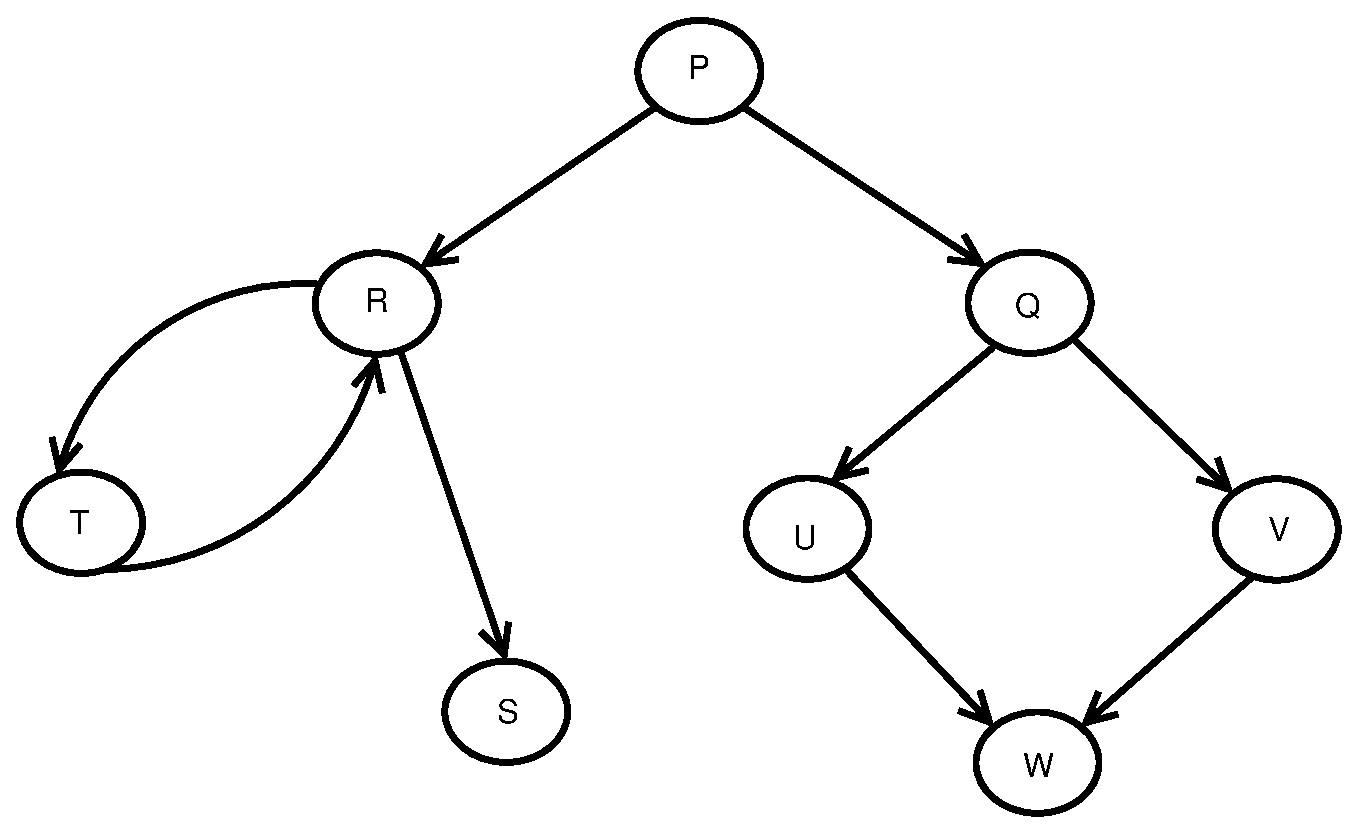
\includegraphics[scale=0.3]{Figures/intro_d1.eps}
   & \\
   \footnotesize Heap Structure & \footnotesize Shape at each heap pointer
   \end{tabular}    
  \end{figure}
}

\subsection{Application}
\frame
{
	\frametitle{\subsecname}
		
	\begin{figure}
  	\begin{center}
  
    \scalebox{.80}{
		\begin{tabular}[htbp]{ | c | c  |}
    	\hline
    	& \multirow{3}{*}{ {\tt
\begin{program}{0}
%  \FL\ \ldots
  \UNL{0} void treeAdd(tree p) \{
  \UNL{1}  if(p == NULL)
  \UNL{2} return;
  \NL{1}     tl = p$\rightarrow$left;
  \NL{1}     \tikz[baseline]{\node[fill=blue!20,anchor=base](t1){treeAdd(tl);};}
  \NL{1}      tr = p$\rightarrow$right;
  \NL{1}     \tikz[baseline]{\node[fill=blue!20,anchor=base](t3){treeAdd(tr);};}
  \UNL{1}	p\rtarrow{num} = tl\rtarrow{num} + tr\rtarrow{num};
  \UNL{0} \}
\end{program}
}
} \\
      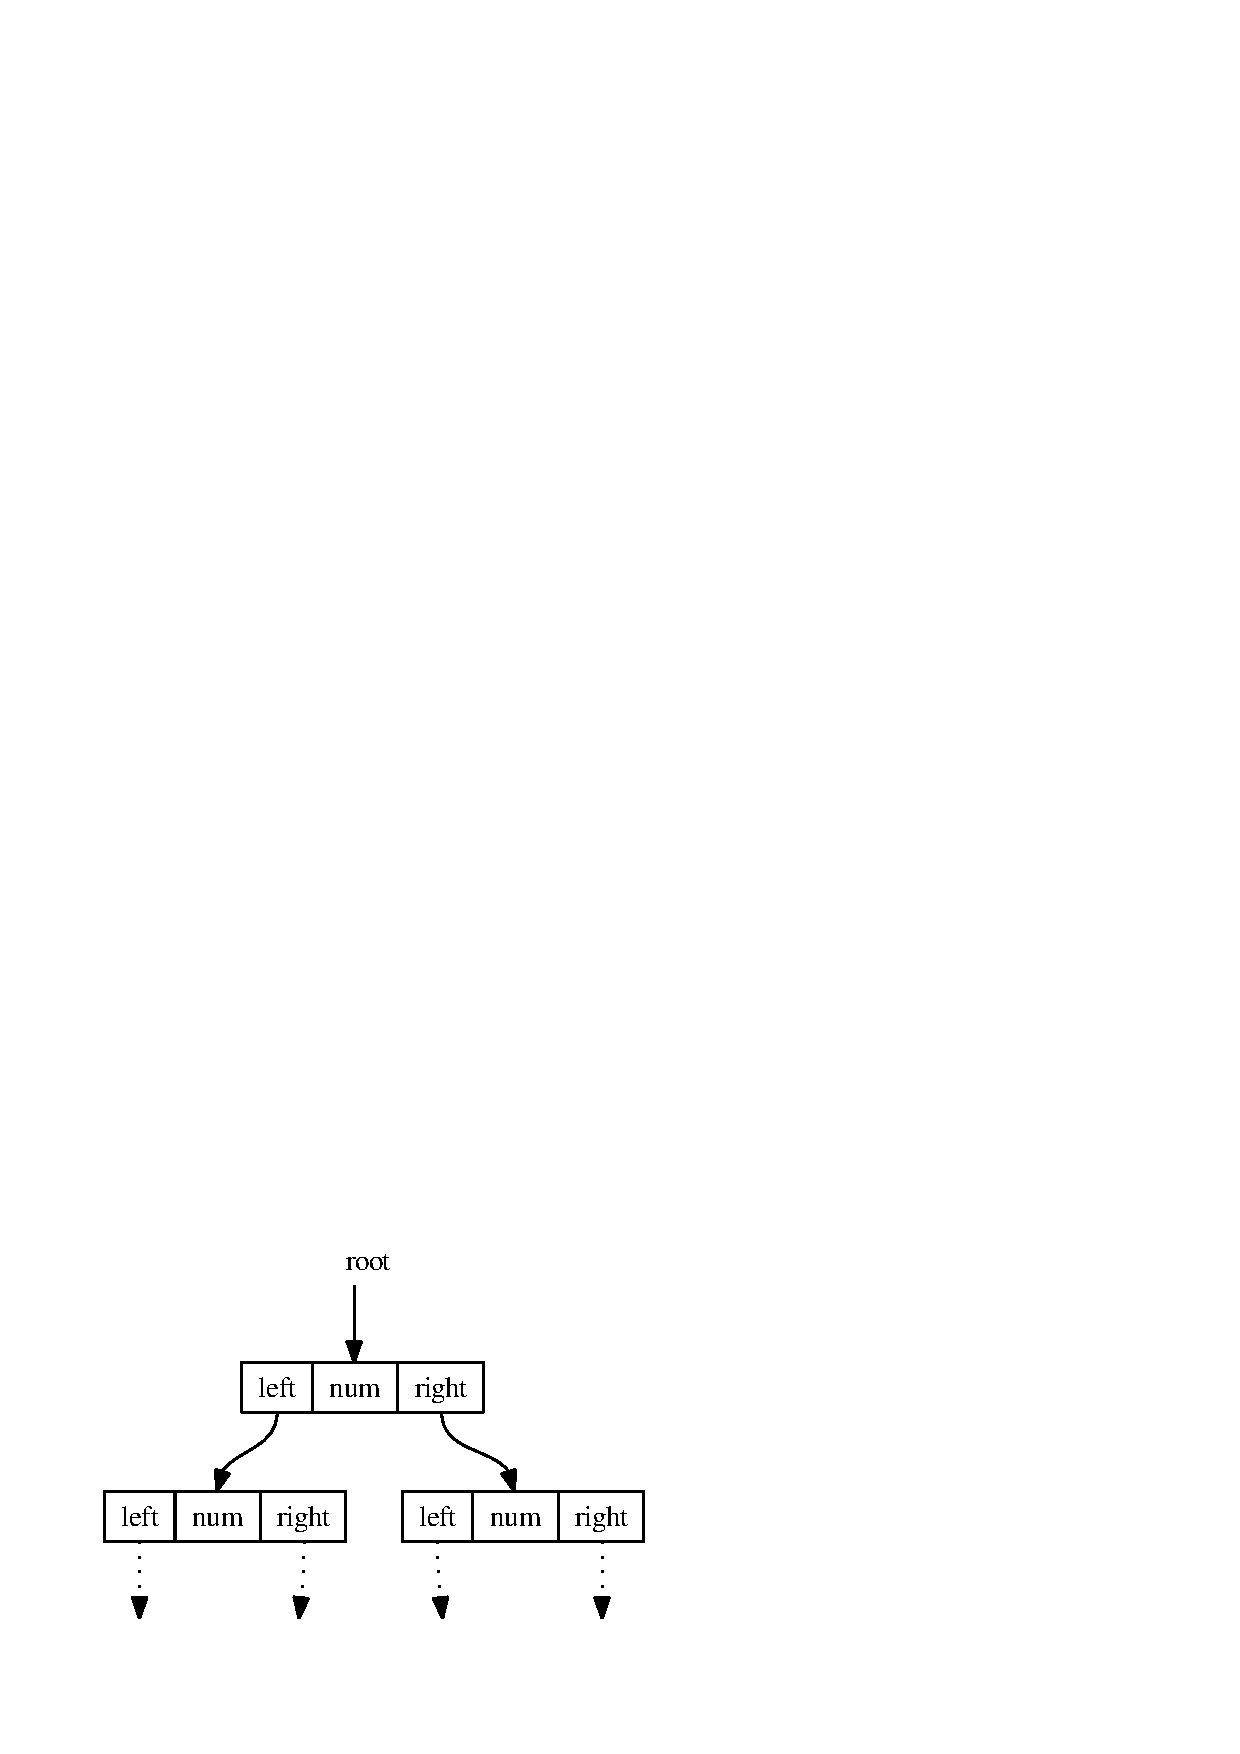
\includegraphics[scale=0.6]{tree_grph}
      & \\
     (a) Heap structure & 
     (b Function traversing the data structure. \\
     \hline
    \end{tabular}
	}
  	\end{center}
	\end{figure}

	\begin{center}
	(p.shape $==$ Tree) $\Rightarrow$ {\tt S2} and {\tt S4} can be executed in parallel.
  	\end{center}
}

\section{Background}

\subsection{Background}
\frame
{
	\frametitle{\subsecname}
	\begin{itemize}
	\item Work done by Ghiya et. al\footnote{Rakesh Ghiya and Laurie J. Hendren. Is it a Tree, a DAG, or a Cyclic graph? 
	a shape analysis for heap-directed pointers in C. In Proceedings of the 23rd ACM
	SIGPLAN-SIGACT symposium on Principles of programming languages, pages 1-15, January 1996.}
	
	\begin{itemize}
	\item Keeps interference and direction matrices between any two 
			pointer variables.
	\item Infer the shape of the structures as Tree, DAG or Cycle
	\item Conservatively identify the shapes.
	\end{itemize}
	\end{itemize}
}

\frame
{
	\frametitle{\subsecname}
	\begin{itemize}
	\item Work done by Sagiv et. al \footnote{Mooly Sagiv, Thomas Reps, and ReinhardWilhelm. Parametric shape analysis via
	3-valued logic. POPL 1999, pages 105-118, 1999.}
	
	\begin{itemize}
	\item Introduce the concepts of abstraction and re-materialization.
	\item Large number of shape nodes may arise. 
	\end{itemize}
	\end{itemize}
		
}

\frame
{

	\frametitle{\subsecname}
	\begin{itemize}
	\item Work done by Marron et. al \footnote{ Mark Marron, Deepak Kapur, Darko Stefanovic, and Manuel Hermenegildo. A
static heap analysis for shape and connectivity: unified memory analysis: the base
framework. LCPC'06, pages 345-363, 2006.} 
	
	\begin{itemize}
	\item Presents a data flow framework that uses heap graphs to model data flow values.
	\item The analysis uses technique similar to re-materialization, but the re-materialization is approximate and 
	may result in loss of precision.
	\end{itemize}
	\end{itemize}
		
}

\subsection{Precise Shape Analysis using Field Sensitivity}

\frame
{
  \frametitle{\subsecname}

  \begin{itemize}
   \item This work was started as an earlier MTech Thesis of Sandeep Dasgupta 
   \item Sandeep Dasgupta and Amey Karkare. Precise shape analysis using field
    sensitivity. In Proceedings of the 27th Annual ACM Symposium on Applied
    Computing, SAC ’12, pages 1300–1307, New York, NY, USA, 2012. ACM
   \item Sandeep Dasgupta. Precise shape analysis using field sensitivity.Technical report, Master’s thesis, IIT Kanpur, 2011.
  \end{itemize}

}
\frame
{
  \frametitle{Precise Shape Analysis using Field Sensitivity}  
   \begin{itemize}
    \item Uses limited field sensitivity to infer the shape of heap. 
	    \begin{eqnarray*}
	  \p \rightarrow \f &=& \q \\ 
	  \q \rightarrow \f &=& \p \\ 
	  \q \rightarrow \f &=& NULL
	  \end{eqnarray*}
    \item Identify the transitions 
    \begin{itemize}
     \item Cycle $\rightarrow$ Dag
     \item Cycle $\rightarrow$ Tree
     \item Dag $\rightarrow$ Tree
    \end{itemize}
    \item Data flow analysis.
    \begin{itemize}
     \item Technique for collecting information at different parts of a program
      \cmt{With the help of CFG they know in which path these set of values are going}
     \item Out[S] = Gen[S] $\bigcup$ (In[S] - Kill[S])
    \end{itemize}

   \end{itemize}
}


% \frame
% {
%     \frametitle{Analysis}
%     
%     \begin{itemize}
%      \item  Heap structure at a program point as a directed graph. \pause
% 	    \begin{itemize}
% 	      \item  {\blue $D_F$}: Direction matrix. \cmt{ that stores the first fields of the paths between two pointers.}
% 	      \pause
% 	      \item {\blue $I_F$}: Interference matrix. \cmt{ that stores the pairs of first fields corresponding to the pairs of interfering paths.}
% 	      \pause
% 	      \item {\blue Boolean Variables}: For $f \in \fields, \p, \q \in \heap$, \\ 
% 			\begin{center}
% 			$f_{pq} = \left\{\begin{array}{@{}ll}
% 			                  \true & \f \ field \ of \  \p \ points \ directly \ to \ \q \\
% 					  \false & Otherwise
% 			                 \end{array}\right.$
% 			\end{center}
% 	    \end{itemize}
% 
%     \end{itemize}
% }

\subsection{Example : $D_F ,I_F \mbox{ and }  f_{pq}$}
\frame
{
	\frametitle{\subsecname}
	\begin{figure}
\centering
\begin{tabular}{c@{$\qquad\qquad$}c}
\psset{unit=1.2mm}
\begin{pspicture}(0,0)(15,20)
	\psset{linecolor=black}
  \putnode{p0}{origin}{3}{9}{\pscirclebox{\p}}
  \putnode{q0}{p0}{5}{7}{\pscirclebox{\q}}
  %\putnode{r0}{p0}{0}{-14}{\pscirclebox{\myr}}
  \putnode{r0}{p0}{10}{0}{\pscirclebox{\myr}}
	\psset{linecolor=black}
  \ncline[nodesep=-.3]{<-}{p0}{q0}
  \aput[0.2](0.4){$\scriptstyle f$}
  \ncline{<-}{p0}{r0}
  \aput[0.2](0.4){$\scriptstyle g$}
%   %\ncline[nodesep=-.5]{->}{s0}{r0}
%   %\aput[0.2](0.2){$\scriptstyle f_5$}
%   \nccurve[angleA=45,angleB=0,linestyle=dotted,dotsep=0.2,ncurv=1,nodesepA=-.8]{->}{p0}{s0}
%   \aput[0.2](0.2){$\scriptstyle f_2$}
%   %\nccurve[angleA=180,angleB=225,linestyle=dotted,dotsep=0.2,ncurv=1,nodesepB=-.5]{->}{q0}{r0}
%   %\bput[0.2](0.2){$\scriptstyle f_4$}
\end{pspicture} &
\scalebox{0.8}{
\renewcommand{\arraystretch}{1.2}
\begin{tabular}[b]{|c|c|c|c|}
\hline
$D_F$          & \p                          & \q                             &  \myr  \\ \hline \hline 
\p 	           & $\{\epsilon\}$              & $\emptyset$            & $\emptyset$     \\ \hline 
\q             & $\{\fieldD{f}{}\}$                  & $\{\epsilon\}$                 & $\emptyset$   \\ \hline
\myr             & $\{\fieldD{g}{}\}$                 & $\emptyset$                    & $\{\epsilon\}$       \\ \hline
\end{tabular}} \\
\scalebox{0.80}{ (a) Heap graph} & \scalebox{0.80}{ (b) Direction Matrix}  \\ \\
% \multicolumn{2}{c}{
& \multirow{6}{*}{
\begin{tabular}{c}
$f_{\q\p} = \true$ \\
$f_{\p\q} = \false$ \\
$g_{\myr\p} = \true$ \\ 
\end{tabular}
} \\

\scalebox{0.80}{
\renewcommand{\arraystretch}{1.2}
\newcommand{\iwd}{0.23\columnwidth}
\begin{tabular}[b]{|c|c|c|c|}
\hline 
$\ I_F$     & $\p$	               & $\q$ &  $\myr$             \\ \hline \hline 
%%
$\p$ & $\{\epsilon, \epsilon\}$    & $\{(\epsilon, \fieldD{f}{}) \}$               & $\{(\epsilon, \fieldD{g}{})\}$      \\      \hline 
%%
$\q$       & $\{(\fieldD{f}{}, \epsilon)\}$                 & $\{\epsilon, \epsilon\}$          & $\{(\fieldD{f}{}, \fieldD{g}{})\}$         \\  \hline              
%%
$\myr$       & $\{(\fieldD{g}{}, \epsilon)\}$             & $\{(\fieldD{g}{}, \fieldD{f}{})\}$             & $\{\epsilon, \epsilon\}$         \\ \hline              
%%
\end{tabular}} &  \\
% } \\
% \multicolumn{2}{c}{\scalebox{0.80}{ (c) Interference Matrix} }
\scalebox{0.80}{(c) Interference Matrix}  & \scalebox{0.80}{(d) Bolean variables}
\end{tabular}
%\caption{A heap graph and its field sensitive path matrices\label{fig:DFM_IFM}}
\end{figure}

}

\subsection{Example with Analysis}
\frame
{
	\frametitle{\subsecname}
	
\begin{figure}
  \begin{center}
  
    \scalebox{.80}{\begin{tabular}{ |@{}l@{ }|@{}c@{}|@{}c@{}|@{}c@{}|@{}c@{}|  }
   \hline
   \multirow{2}{*}{Statements} & \multirow{2}{*}{Heap Structure} & \multirow{2}{*}{Boolean Functions} &  \multicolumn{2}{@{}c@{}|}{Shape Inference}  \\
   \cline{4-5} 
   &  &  &   p.shape & q.shape  \\
   \hline
	 &&&& \\
    {\tt S1.} \ttf{p = malloc()} & \multirow{2}{*}{\begin{pspicture}(0,3)(3,4.2)
\psset{linecolor=blue}
\pscircle(.7,3.6){.3}
\pscircle(2.3,3.6){.3}
\rput(2.3,3.6){\psframebox*{\scalebox{.8}{\ttf{q}}}}
\rput(.7,3.6){\psframebox*{\scalebox{.8}{\ttf{p}}}}
\end{pspicture}
} &  
																				$\begin{array}{@{}c@{}}
																					p_{\subC} = \false  \qquad q_{\subC} = \false \\ 
																					p_{\subD} = \false  \qquad q_{\subD} = \false 
																				\end{array}$
																				& \multirow{2}{*}{Tree} & \multirow{2}{*}{Tree} \\
    {\tt S2.} \ttf{q = malloc()} &    &&&\\
	 &&&& \\
    \hline
	\pause
	 &&&& \\
	{\tt S3.} \ttf{p$\rightarrow$f = q} &  \begin{pspicture}(0,3)(3,4.2)
\psset{linecolor=blue}
\pscircle(.7,3.6){.3}
\pscircle(2.3,3.6){.3}
\psset{linecolor=black}
\psline[linewidth=1pt,linearc=.5]{->}(1.0,3.6)(1.5, 3.9)(2.0,3.6)
\rput(2.3,3.6){\psframebox*{\scalebox{.8}{\ttf{q}}}}
\rput(1.5,4.1){\psframebox*{\scalebox{.8}{\ttf{f}}}}
\rput(.7,3.6){\psframebox*{\scalebox{.8}{\ttf{p}}}}
\end{pspicture}
 & 
																				$\begin{array}{@{}c@{}}
																					p_{\subC} = (f_{\p\q} \wedge \num{D_F[q,p]} \geq 1) \\ \\
																					q_{\subC} = f_{\p\q} \wedge \num{D_F[q,p]} \geq 1 \\ \\
% 																					p_{\subD} = f_{\p\q} \wedge \num{I_F[\p,\q]} > 1 \\ \\
																					f_{\p\q} = \true
																				\end{array}$
																	  & Tree & Tree\\
	 &&&& \\
     \hline
	\pause
	 &&&& \\
	{\tt S4.} \ttf{q$\rightarrow$f = p} &  \begin{pspicture}(0,3)(3,4.2)
\psset{linecolor=blue}
\pscircle(.7,3.6){.3}
\pscircle(2.3,3.6){.3}
\psset{linecolor=black}
\psline[linewidth=1pt,linearc=.5]{->}(1.0,3.6)(1.5, 3.9)(2.0,3.6)
\psline[linewidth=1pt,linearc=.5]{<-}(1.0,3.6)(1.5, 3.3)(2.0,3.6)
\rput(2.3,3.6){\psframebox*{\scalebox{.8}{\ttf{q}}}}
\rput(1.5,4.1){\psframebox*{\scalebox{.8}{\ttf{f}}}}
\rput(1.5,3.1){\psframebox*{\scalebox{.8}{\ttf{f}}}}
\rput(.7,3.6){\psframebox*{\scalebox{.8}{\ttf{p}}}}
\end{pspicture}
 & 
																				$\begin{array}{@{}c@{}}
																					\p_{\subC} = (f_{\q\p} \wedge \num{D_F[p,q]} \geq 1) \\ \\
																					\q_{\subC} = (f_{\q\p} \wedge \num{D_F[p,q]} \geq 1) \\ \\    
																					f_{\p\q} = \true \qquad f_{\q\p} = \true
																				\end{array}$
																	  & Cycle & Cycle\\
	 
     \hline
    \end{tabular}}
  \end{center}
\end{figure}
}

\frame
{
  \frametitle{\subsecname}
	
\begin{figure}
  \begin{center}
  
    \scalebox{.80}{\begin{tabular}{ |@{}l@{ }|@{}c@{}|@{}c@{}|@{}c@{}|@{}c@{}|  }
   \hline
   \multirow{2}{*}{Statements} & \multirow{2}{*}{Heap Structure} & \multirow{2}{*}{Boolean Functions} &  \multicolumn{2}{@{}c@{}|}{Shape Inference}  \\
   \cline{4-5} 
   &  &  &   p.shape & q.shape  \\
   \hline
   {\tt S4.} \ttf{q$\rightarrow$f = NULL} &  \begin{pspicture}(0,3)(3,4.2)
\psset{linecolor=blue}
\pscircle(.7,3.6){.3}
\pscircle(2.3,3.6){.3}
\psset{linecolor=black}
\psline[linewidth=1pt,linearc=.5]{->}(1.0,3.6)(1.5, 3.9)(2.0,3.6)
\rput(2.3,3.6){\psframebox*{\scalebox{.8}{\ttf{q}}}}
\rput(1.5,4.1){\psframebox*{\scalebox{.8}{\ttf{f}}}}
\rput(.7,3.6){\psframebox*{\scalebox{.8}{\ttf{p}}}}
\end{pspicture}
 & 
																				$\begin{array}{@{}c@{}}
																					\p_{\subC} = (f_{\q\p} \wedge \num{D_F[p,q]} \geq 1) \\ \\
																					\q_{\subC} = (f_{\q\p} \wedge \num{D_F[p,q]} \geq 1) \\ \\    
																					f_{\p\q} = \true \qquad f_{\q\p} = \false
																				\end{array}$
																	  & Tree & Tree\\
    \hline
    \end{tabular}}
  \end{center}
\end{figure}
}




\section{Enhancements} 
% How were you able to find out these ??? Tell about Testing strategy
\subsection{Enhancements}
\frame
{
	\frametitle{\subsecname}
	
\begin{figure}
  \begin{center}
  
    \scalebox{.80}{\begin{tabular}{ |@{}l@{ }|@{}c@{}|@{}c@{}|@{}c@{}|@{}c@{}|  }
   \hline
   \multirow{2}{*}{Statements} & \multirow{2}{*}{Heap Structure} & \multirow{2}{*}{Boolean Functions} &  \multicolumn{2}{@{}c@{}|}{Shape Inference}  \\
   \cline{4-5} 
   &  &  &   p.shape & q.shape  \\
   \hline
        
	 &&&& \\
	{\tt S3.} \ttf{p$\rightarrow$f = q} &  \begin{pspicture}(0,3)(3,4.2)
\psset{linecolor=blue}
\pscircle(.7,3.6){.3}
\pscircle(2.3,3.6){.3}
\psset{linecolor=black}
\psline[linewidth=1pt,linearc=.5]{->}(1.0,3.6)(1.5, 3.9)(2.0,3.6)
\rput(2.3,3.6){\psframebox*{\scalebox{.8}{\ttf{q}}}}
\rput(1.5,4.1){\psframebox*{\scalebox{.8}{\ttf{f}}}}
\rput(.7,3.6){\psframebox*{\scalebox{.8}{\ttf{p}}}}
\end{pspicture}
 & 
																				$\begin{array}{@{}c@{}}
																					p_{\subC} = (f_{\p\q} \wedge \num{D_F[q,p]} \geq 1) \\ \\
																					q_{\subC} = f_{\p\q} \wedge \num{D_F[q,p]} \geq 1 \\ \\
% 																					p_{\subD} = f_{\p\q} \wedge \num{I_F[\p,\q]} > 1 \\ \\
																					f_{\p\q} = \true
																				\end{array}$
																	  & Tree & Tree\\
	 &&&& \\
     \hline

	 &&&& \\
	{\tt S4.} \ttf{q$\rightarrow$f = p} &  \begin{pspicture}(0,3)(3,4.2)
\psset{linecolor=blue}
\pscircle(.7,3.6){.3}
\pscircle(2.3,3.6){.3}
\psset{linecolor=black}
\psline[linewidth=1pt,linearc=.5]{->}(1.0,3.6)(1.5, 3.9)(2.0,3.6)
\psline[linewidth=1pt,linearc=.5]{<-}(1.0,3.6)(1.5, 3.3)(2.0,3.6)
\rput(2.3,3.6){\psframebox*{\scalebox{.8}{\ttf{q}}}}
\rput(1.5,4.1){\psframebox*{\scalebox{.8}{\ttf{f}}}}
\rput(1.5,3.1){\psframebox*{\scalebox{.8}{\ttf{f}}}}
\rput(.7,3.6){\psframebox*{\scalebox{.8}{\ttf{p}}}}
\end{pspicture}
 & 
																				$\begin{array}{@{}c@{}}
																					\p_{\subC} = (f_{\q\p} \wedge \num{D_F[p,q]} \geq 1) \\ \\
																					\q_{\subC} = (f_{\q\p} \wedge \num{D_F[p,q]} \geq 1) \\ \\    
																					f_{\p\q} = \true \qquad f_{\q\p} = \true
																				\end{array}$
	
																      & Cycle & Cycle\\
	\hline
	 &&&& \\
	{\tt S5.} \ttf{p = NULL} &  \begin{pspicture}(0,3)(3,4.2)
\psset{linecolor=blue}
\pscircle(.7,3.6){.3}
\pscircle(2.3,3.6){.3}
\psset{linecolor=black}
\psline[linewidth=1pt,linearc=.5]{->}(1.0,3.6)(1.5, 3.9)(2.0,3.6)
\psline[linewidth=1pt,linearc=.5]{<-}(1.0,3.6)(1.5, 3.3)(2.0,3.6)
\rput(2.3,3.6){\psframebox*{\scalebox{.8}{\ttf{q}}}}
\rput(1.5,4.1){\psframebox*{\scalebox{.8}{\ttf{f}}}}
\rput(1.5,3.1){\psframebox*{\scalebox{.8}{\ttf{f}}}}
% \rput(.7,3.6){\psframebox*{\scalebox{.8}{\ttf{p}}}}
\end{pspicture}
 	& 
																				$\begin{array}{@{}c@{}}
																					\p_{\subC} = False \\ \\
																					\q_{\subC} = (f_{\q\p} \wedge \num{D_F[p,q]} \geq 1) \\ \\
																					f_{\p\q} = \false \qquad f_{\q\p} = \false  
																				\end{array}$
	
																		&  Tree & \red{ Tree }\\
     \hline
    \end{tabular}}
  \end{center}
\end{figure}
}
\frame
{
	\frametitle{\subsecname}	

 \centering
Gen, Kill information for \ttf{p = NULL}
\newline
\newline
\centering
 \scalebox{0.80}{
  \begin{tabular}{llll}
	  \KillC{p}  = \InC{p} & \KillD{p} = \InD{p} & \GenC{p} = \false & \GenD{p} = \false \\ \\
	   $\forall \s \in \heap,  s \not= p $ &&& \\ \\
           $f_{\p\s} = \false$  &  $f_{\s\p} = \false$ && \\  \\
	  \red{$D_F^{\dkill}[\p,\s]$  =  $D_F^{\din}[\p,\s]$} & \red{$D_F^{\dkill}[\s,\p]$  =  $D_F^{\din}[\s,\p]$} & $D_F^{\dgen}[\p,\s]$    =  $\emptyset$  & $D_F^{\dgen}[\s,\p]$    =  $\emptyset$ \\ \\
	  $I_F^{\dkill}[\p,\s]$  =  $I_F^{\din}[\p,\s]$ && $I_F^{\dgen}[\p,\s]$    =  $\emptyset$  &
  \end{tabular}
}

}

\frame
{  
 \frametitle{Solution}

\begin{itemize}
 \item Killing information even when graph structure is not changing. 
 \item Preserve information about unlabeled node. 
 \item Create a dummy pointer $\delta$, pointing to the node pointed by p before statement $\p=NULL$. \\
	\centering \begin{pspicture}(0,3)(3,4.2)
\psset{linecolor=blue}
\pscircle(.7,3.6){.3}
\pscircle(2.3,3.6){.3}
\psset{linecolor=black}
\psline[linewidth=1pt,linearc=.5]{->}(1.0,3.6)(1.5, 3.9)(2.0,3.6)
\psline[linewidth=1pt,linearc=.5]{<-}(1.0,3.6)(1.5, 3.3)(2.0,3.6)
\rput(2.3,3.6){\psframebox*{\scalebox{.8}{\ttf{q}}}}
\rput(1.5,4.1){\psframebox*{\scalebox{.8}{\ttf{f}}}}
\rput(1.5,3.1){\psframebox*{\scalebox{.8}{\ttf{f}}}}
\rput(.7,3.6){\psframebox*{\scalebox{.8}{\ttf{$\delta$}}}}
\end{pspicture}
 \end{itemize}
 \begin{itemize}
 \item Before the statement $\p=NULL$, a statement $\delta = \p$ is inserted which has no kill information.
 \item Replace all information regarding $p$ with $\delta$ at this new statement.  
 \end{itemize}
 
}

\frame
{
	\frametitle{\subsecname}	
\begin{figure}
  \begin{center}  
    \scalebox{.80}{\begin{tabular}{ |@{}l@{ }|@{}c@{}|@{}c@{}|@{}c@{}|@{}c@{}|  }
   \hline
   \multirow{2}{*}{Statements} & \multirow{2}{*}{Heap Structure} & \multirow{2}{*}{Boolean Functions} &  \multicolumn{2}{@{}c@{}|}{Shape Inference}  \\
   \cline{4-5} 
   &  &  &   p.shape & q.shape  \\
     \hline
	 &&&& \\
      {\tt S4.} \ttf{q$\rightarrow$f = p} &  \begin{pspicture}(0,3)(3,4.2)
\psset{linecolor=blue}
\pscircle(.7,3.6){.3}
\pscircle(2.3,3.6){.3}
\psset{linecolor=black}
\psline[linewidth=1pt,linearc=.5]{->}(1.0,3.6)(1.5, 3.9)(2.0,3.6)
\psline[linewidth=1pt,linearc=.5]{<-}(1.0,3.6)(1.5, 3.3)(2.0,3.6)
\rput(2.3,3.6){\psframebox*{\scalebox{.8}{\ttf{q}}}}
\rput(1.5,4.1){\psframebox*{\scalebox{.8}{\ttf{f}}}}
\rput(1.5,3.1){\psframebox*{\scalebox{.8}{\ttf{f}}}}
\rput(.7,3.6){\psframebox*{\scalebox{.8}{\ttf{p}}}}
\end{pspicture}
 & 
																				$\begin{array}{@{}c@{}}
																					\p_{\subC} = (f_{\q\p} \wedge \num{D_F[p,q]} \geq 1) \\ \\
																					\q_{\subC} = (f_{\q\p} \wedge \num{D_F[p,q]} \geq 1) \\ \\    
																					f_{\p\q} = \true \qquad f_{\q\p} = \true
																				\end{array}$
																	  & Cycle & Cycle\\ \hline	
	 &&&& \\
																		
        \ \ttf{ $\delta$ = p } & \begin{pspicture}(0,3)(3,4.2)
\psset{linecolor=blue}
\pscircle(.7,3.6){.3}
\pscircle(2.3,3.6){.3}
\psset{linecolor=black}
\psline[linewidth=1pt,linearc=.5]{->}(1.0,3.6)(1.5, 3.9)(2.0,3.6)
\psline[linewidth=1pt,linearc=.5]{<-}(1.0,3.6)(1.5, 3.3)(2.0,3.6)
\rput(2.3,3.6){\psframebox*{\scalebox{.8}{\ttf{q}}}}
\rput(1.5,4.1){\psframebox*{\scalebox{.8}{\ttf{f}}}}
\rput(1.5,3.1){\psframebox*{\scalebox{.8}{\ttf{f}}}}
\rput(.7,3.6){\psframebox*{\scalebox{.8}{\ttf{$\delta$}}}}
\end{pspicture}   &
																				$\begin{array}{@{}c@{}}
																					\p_{\subC} = (f_{\q\delta} \wedge \num{D_F[\delta,q]} \geq 1) \\ \\
																					\q_{\subC} = (f_{\q\delta} \wedge \num{D_F[\delta,q]} \geq 1) \\ \\
																					f_{\delta\q} = \true \qquad f_{\q\delta} = \true  
																				\end{array}$ 
	&  Cycle & Cycle\\
	\hline
	
	{\tt S5.} \ttf{p = NULL} &  \begin{pspicture}(0,3)(3,4.2)
\psset{linecolor=blue}
\pscircle(.7,3.6){.3}
\pscircle(2.3,3.6){.3}
\psset{linecolor=black}
\psline[linewidth=1pt,linearc=.5]{->}(1.0,3.6)(1.5, 3.9)(2.0,3.6)
\psline[linewidth=1pt,linearc=.5]{<-}(1.0,3.6)(1.5, 3.3)(2.0,3.6)
\rput(2.3,3.6){\psframebox*{\scalebox{.8}{\ttf{q}}}}
\rput(1.5,4.1){\psframebox*{\scalebox{.8}{\ttf{f}}}}
\rput(1.5,3.1){\psframebox*{\scalebox{.8}{\ttf{f}}}}
\rput(.7,3.6){\psframebox*{\scalebox{.8}{\ttf{$\delta$}}}}
\end{pspicture} 	& 
																				$\begin{array}{@{}c@{}}
																					\p_{\subC} = False \\ \\
																					\q_{\subC} = (f_{\delta\q} \wedge \num{D_F[q,\delta]} \geq 1) \\ \\
																					f_{\delta\q} = \true   
																				\end{array}$
	&  Tree & \blue{ Cycle }\\
																						
	\hline
    \end{tabular}}
  \end{center}
\end{figure}

}

\frame
{
  \frametitle{\subsecname}
  \begin{itemize}
   \item Information Passed to Successors
      \begin{itemize}
       \item A boolean function is passed to its successor only if it evaluates to \true. 	
       \item Boolean function generated at each statement is itself capable of detecting the shape transition at that point. 
       \item Increase in precision for programs involving control structures.
       \item Memory consumption is reduced.
      \end{itemize}
  \item Modified the data flow equations
  \begin{itemize}
  \item Handling of Aliases.       
  \item	 Better approximations to increase precision.
	\begin{itemize}
	 \item p = q $\rightarrow$ f 
	\end{itemize}
  \end{itemize}
  \end{itemize}
}

\section{Subset Based Analysis}
\subsection{Subset Based Analysis}
\frame
{
  \frametitle{\subsecname}
    
  \begin{itemize}
   \item Auxiliary fields in data structures.
   \item Searching in a Tree which has an auxiliary Parent field (red).
  \end{itemize}
    \centering \includegraphics[scale=0.4]{tree.eps}   
   \begin{itemize}
     \pause
    \item Conservative shape(Cycle) is obtained.   
    \item Parent is used for debugging , not for the core algorithm.
    \item Shape should be inferred as Tree here.
   \end{itemize}
}

\subsection{Analysis}
\frame
{
  \frametitle{\subsecname}
%    \centering 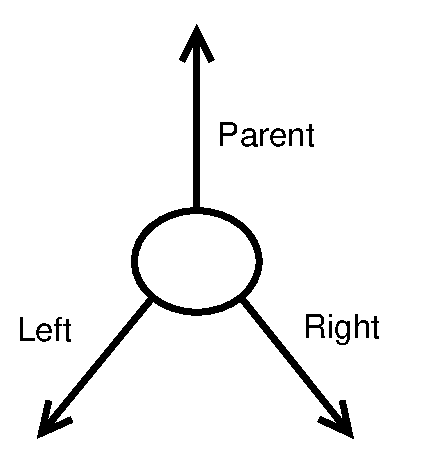
\includegraphics[scale=0.2]{Figures/node_subset.eps}

    \begin{itemize}
     \item $S_{F}$ : Subset of fields accessed by function $F$.
      \begin{center}
      $S_{insert}$ = \{ Left , {\blue{Right}} , {\red{Parent}} \} \\
      $S_{search}$ = \{ Left , {\blue{Right}} \} \\ 
      \end{center}

\pause
      \item The terms $f_{\p\q}$,\ $D[\p, \q]$,\ $I[\p, \q]$ are replaced by the the terms $f_{\p\q}^{\#} , {D^{\#}[p,q]} ,{I^{\#}[p,q]}$ respectively.             
   \end{itemize}
   
% \begin{center}
% \begin{tabular}{ccc}
% $f_{\p\q}^{\#}$ & = & $\left \{ \begin{array}{@{}ll}
%                        f_{\p\q}  & \f \in S_F  \\
% 			 \false & \mbox{Otherwise}
%                        \end{array} \right.$ \\ \\
% $D^{\#}[\p, \q]$ & = & $D[\p, \q] -\bigcup_{ \f \in \fields,\f \not \in S_F } \ \{  \project{D[\p,\q]}{f}         \}$ \\ \\
% $I^{\#}[\p, \q]$ & = & $I[\p, \q] - \bigcup_{ \f \in \fields,\f \not \in S_F } \ \{  \project{I[\p,\q]}{f}         \}$ \\ \\
% \end{tabular}
% \end{center}

\begin{center}
\begin{tabular}{ccc}
$f_{\p\q}^{\#}$ & = & $\left \{ \begin{array}{@{}ll}
                       f_{\p\q}  & \f \in S_F  \\
			 \false & \mbox{Otherwise}
                       \end{array} \right.$ \\ \\
$D^{\#}[\p, \q]$ & = & $D[\p, \q] - \f^{*} $ \\ \\
$I^{\#}[\p, \q]$ & = & $I[\p, \q] - \{ \f^{*}, \f^{*} \}$ \\ \\
\end{tabular}
\end{center}



% \begin{center}
% \begin{tabular}{ccc}
% $D^{\#}[\p, \q]$ & = & $D[\p, \q] -\bigcup_{ \f \in \fields,\f \not \in S_F } \{  \project{D[\p,\q]}{f}         \}$ \\ \\
% $I^{\#}[\p, \q]$ & = & $I[\p, \q] - \bigcup_{ \f \in \fields,\f \not \in S_F } \{  \project{I[\p,\q]}{f}         \}$ \\ \\
% $f_{\p\q}^{\#}$ & = & $\left \{ \begin{array}{@{}ll}
%                        f_{\p\q}  & \f \in S_F  \\
% 			 \false & \mbox{Otherwise}
%                        \end{array} \right.$
% \end{tabular}
% \end{center}


}

\frame
{
  \begin{itemize}
   \item Heap graph view in each function. \\
  \end{itemize}
    
    \begin{table}
    \begin{tabular}{cc}
     \includegraphics[scale=0.4]{tree.eps}  & \includegraphics[scale=0.4]{tree1.eps}  \\
     Insert & Search      
    \end{tabular}
%     \caption{Heap graph viewed in the functions}
    \end{table}
  
}



% \frame
% {
%     \frametitle{\subsecname}
%     
%   \begin{itemize}
%   \item Increases the precision at the cost of extra computation.
%   \item 
%   \end{itemize}
%   
%   
% }

\section{Inter Procedural Analysis}

\subsection{Inter Procedural Analysis}
\frame
{
  \frametitle{\subsecname}
  \begin{itemize}
   \item In Intra Procedural Analysis worst case assumptions are to be made. \pause
   \item Variants of Inter Procedural Analysis \\
	\begin{itemize}
	 \item Context Sensitive
	\end{itemize}
	\centering  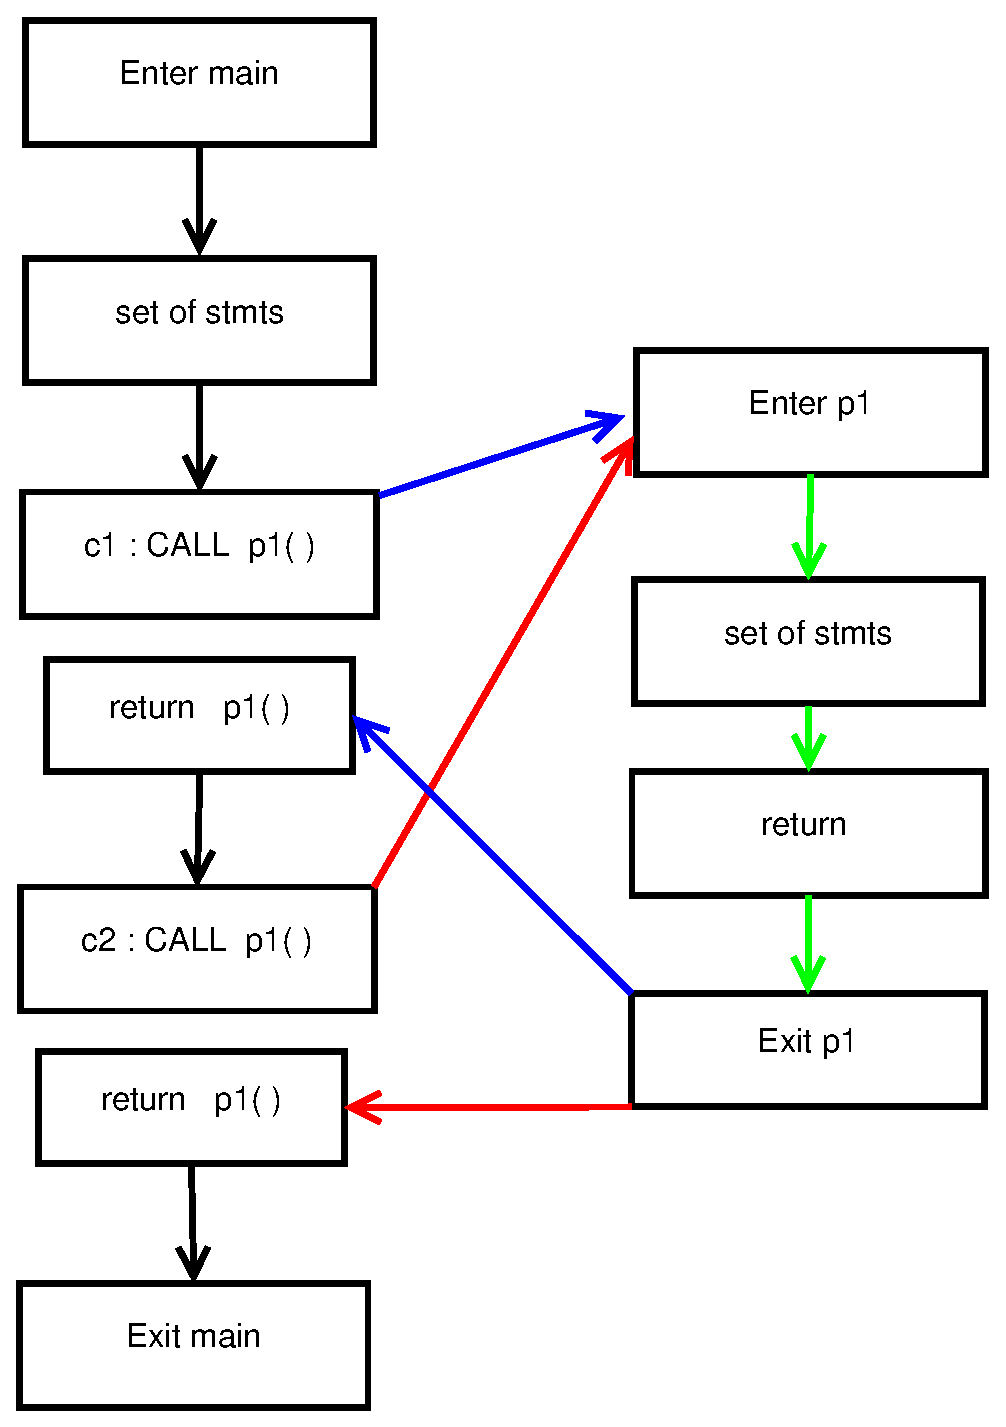
\includegraphics[scale=0.25]{Figures/Diagram1.eps}                 
  \end{itemize}

}

\frame
{
  \frametitle{\subsecname}
  \begin{itemize}
   \item In Intra Procedural Analysis worst case assumptions are to be made. 
   \item Variants of Inter Procedural Analysis \\
	\begin{itemize}
	 \item Context Sensitive
	 \item Context Insensitive 
	\end{itemize}
	\centering  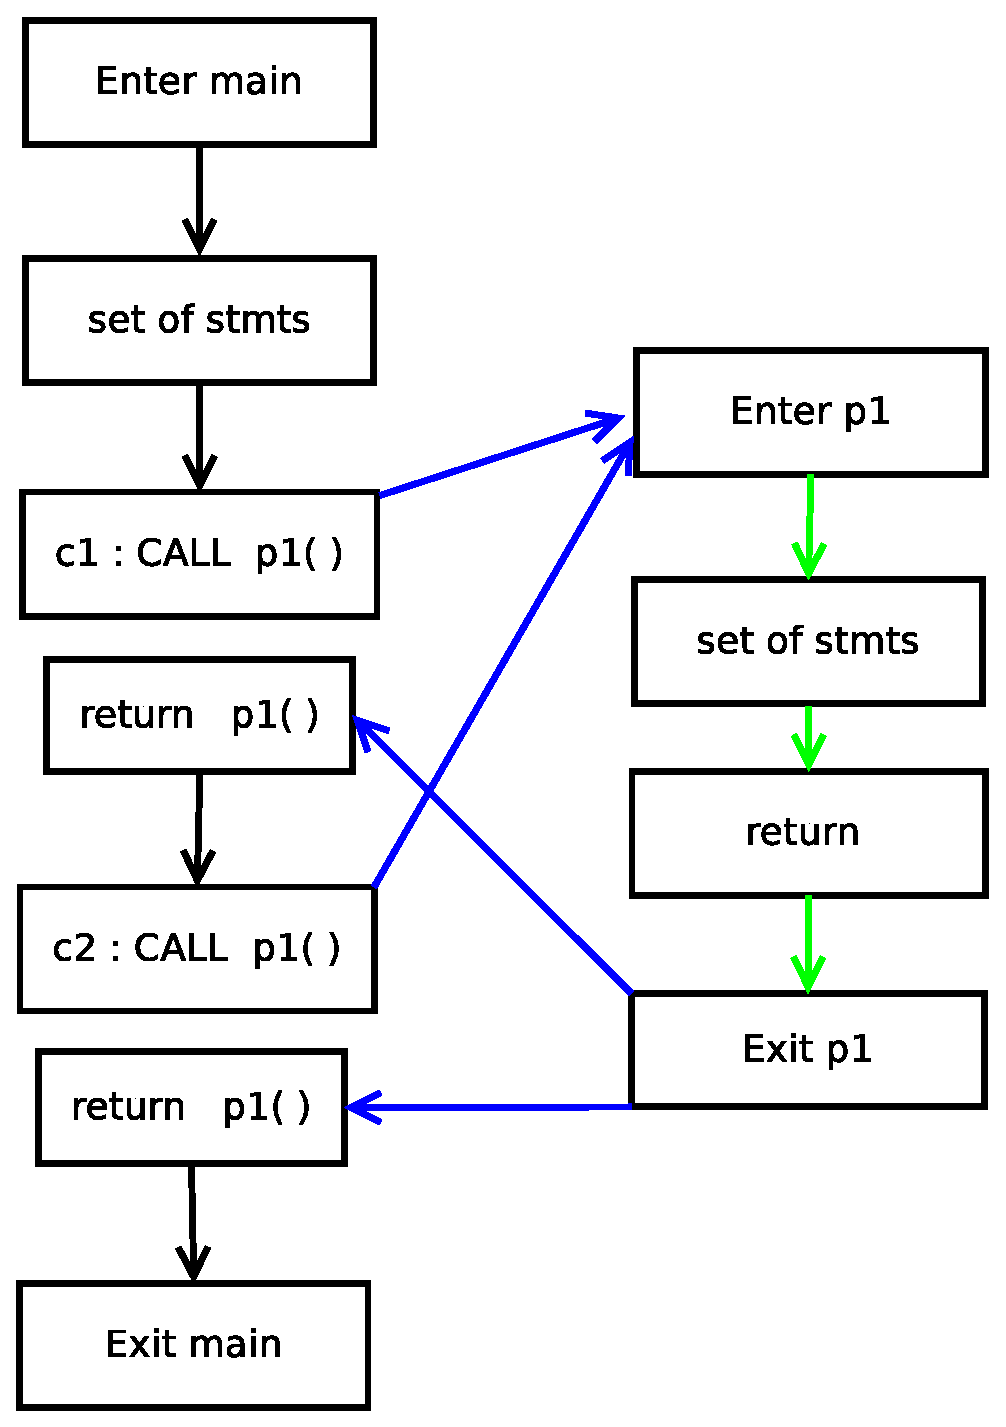
\includegraphics[scale=0.25]{Figures/Diagram2.eps}                 
  \end{itemize}

}

\frame
{
  \frametitle{\subsecname}
   \centering  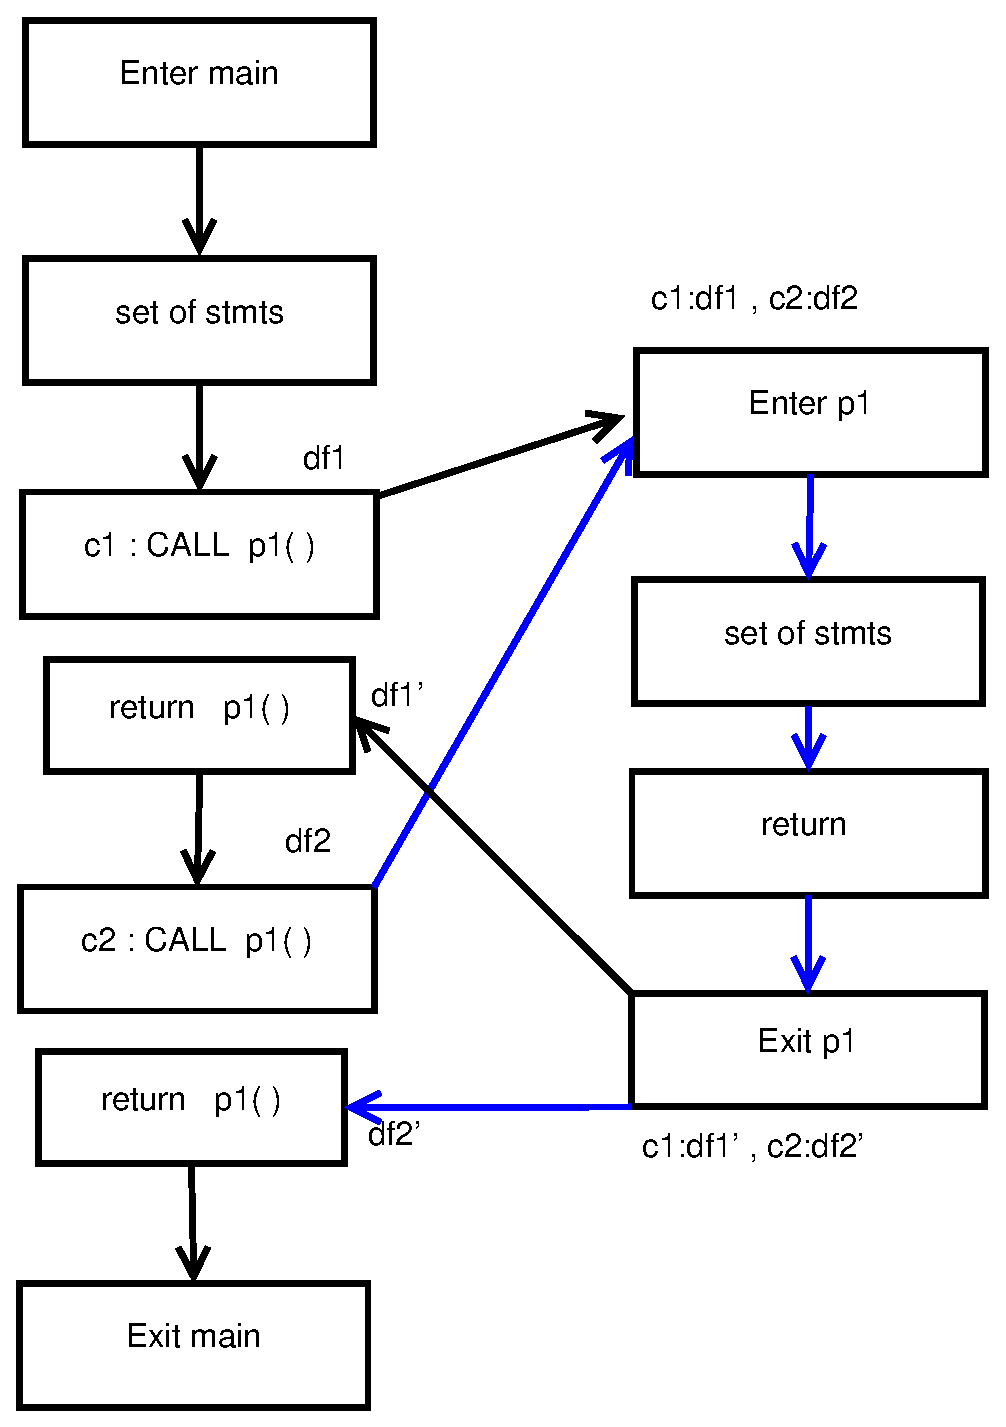
\includegraphics[scale=0.25]{Figures/Diagram12.eps}                  
   \begin{itemize}
    \item Callstring based approach	
	\begin{itemize}
	\item $<$ Call String cs: Data Flow value d $>$
	\item Separate set of dataflow values for each call string
	\item Memory usage
	\end{itemize}    
   \end{itemize}  
}

\subsection{Shape Sensitive}
\begin{frame}[fragile]
  \frametitle{\subsecname}
  \begin{itemize}
   \item Middleway of Context Sensitive and Context Insensitive \pause
   \item Compromise between memory and accuracy \pause
   \item Based on the shape of the heap pointer arguments of the function call, the merging of contexts takes place.\pause
   \item Implementation is not done for this analysis yet.
  \end{itemize}
\end{frame}


\section{Implementation,Testing and Results}
\subsection{Implementation}

\lstset{basicstyle=\normalsize}

\begin{frame}[fragile]

\frametitle{\subsecname}

\begin{itemize}
 \item Implemented as a plugin for GCC.
 \item High level flow of the implementation. 
\end{itemize}

\begin{center}
% \scalebox{0.80}{
\begin{tabular}{c} 
\begin{lstlisting}
		begin
		  gatherHeapAndFieldPointers();
		  preprocessCFG();  
		  shapeAnalysis();
		  restoreCFG();
		end
\end{lstlisting} 
\end{tabular}
% }
\cmt{optimizations done}
\end{center}
\end{frame}

\lstset{basicstyle=\scriptsize}

\subsection{Testing}

\begin{frame}[fragile]
  \frametitle{\subsecname}
  \begin{itemize}
   \item Generated Unit test cases depending on number of heap manipulation statements 
  \end{itemize}

\begin{center}
\begin{tabular}{ll}

\begin{tabular}{c} 
\begin{lstlisting}
#include <stdlib.h>
int main()
{
	 typedef struct _node node;
	 struct _node {
		 node* f;
		 node* g;
	};

	 node* p = (node*)malloc(sizeof(node));
	 node* q = (node*)malloc(sizeof(node));

	/* HEAP MANIPULATION STARTS */
	.......
	.......
	/* HEAP MANIPULATION ENDS   */
}
\end{lstlisting}
\end{tabular}
&
\scalebox{0.80}{
\begin{tabular}{|c|c|}
 \hline
 {\bf No Of Stmts} & {\bf TestCases Generated} \\ \hline
  1  & 42 \\ \hline
  2  & 1764 \\ \hline
  3  & 74088 \\ \hline 
\end{tabular}
} \\
\end{tabular}
\end{center}

\end{frame}

\frame
{
\frametitle{\subsecname}

 \begin{itemize}
 \item PASS : Ghiya's analysis and our analysis gives the shape information at all statements \pause
 \item SAFE : Ghiya's analysis is more accurate than us, .i.e for example if our analysis infers the shape as CYCLE, then Ghiya will 
 infer more precise shapes like DAG or Tree. \pause
 \item FAIL/ACCURATE : Our analysis gives less conservative shapes than Ghiya. If this happens then there could be two scenarios: 
 either we are giving accurate results or we are giving incorrect results. 
 All the test cases present in this case  are checked manually we ensure that we are not getting any fail cases.
\end{itemize}

}

\subsection{Results}
\frame
{
    \frametitle{Results}
     Unit test case results: Before and after the enhancements

\begin{table} 
\centering
\begin{tabular}{|c@{}|@{}c@{}|@{}c@{}|@{}c@{}|@{}c|}
 \hline
& TestCases & Pass & Safe & Accurate \\ \hline
Before \  & 
\begin{tabular}{c}
  ml-1 \\
  ml-2 \\
  ml-2-if \\
  ml-2-while \\
  ml-3
\end{tabular}
&
\begin{tabular}{c}
 42\\
 1572 \\
 1764 \\
 1108 \\
 51854
\end{tabular}
&
\begin{tabular}{c}
 0 \\
 24 \\
 0 \\
 452 \\
 6864
\end{tabular}
&
\begin{tabular}{c}
 0 \\
 168 \\
 0 \\
 204 \\
 15370
\end{tabular}
\\  \hline%----after
After & 
\begin{tabular}{c}
  ml-1 \\
  ml-2 \\
  ml-2-if \\
  ml-2-while \\
  ml-3 
\end{tabular}
&
\begin{tabular}{c}
  42\\
 1612 \\
 1764 \\
 1452 \\
 58444
\end{tabular}
&
\begin{tabular}{c}
 0\\
 0 \\
 0 \\
 0 \\
 0 
\end{tabular}
&
\begin{tabular}{c}
 0 \\
 152 \\
 0 \\
 312 \\
 16202
\end{tabular}
\\ \hline
\end{tabular}
\end{table}
}

\frame
{
  \frametitle{\subsecname}
  \begin{itemize}
 \item Results when ran on List Benchmarks \footnote{Viktor Pavlu. Basic operations on linked lists (c++), 2010.
http://www.complang.tuwien.ac.at/vpavlu/2010/list-benchmark.tgz} 
 \item   (Tree,Dag,Cycle)
\end{itemize}

  \begin{table}[htbp]
\scalebox{0.70}{
\begin{tabular}{|l|l|c|l|c|c|}
\hline
\multicolumn{ 1}{|c|}{Benchmark} & \multicolumn{ 2}{c|}{Ghiya's Analysis} & \multicolumn{ 2}{c|}{Field Sensitive} & \multicolumn{ 1}{l|}{Result} \\ \cline{ 2- 5}
\multicolumn{ 1}{|c|}{} & Shape & \multicolumn{1}{l|}{Time(Sec)} & Shape & \multicolumn{1}{l|}{Time(Sec)} & \multicolumn{ 1}{l|}{} \\ \hline
100\_create\_iter.cpp & (30,0,0) & 0 & (30,0,0) & 0.179 &  \\ \hline
\red{100\_create\_recur.cpp} & (36,0,0) & 0 & (22,0,14) & 0.147 & \# \\ \hline
200\_delall\_iter\_create\_fixed.cpp & (168,0,0) & 0 & (168,0,0) & 1.385 &  \\ \hline
200\_delall\_iter\_create\_iter.cpp & (63,0,0) & 0 & (63,0,0) & 0.644 &  \\ \hline
200\_delall\_recur\_create\_fixed.cpp & (12,0,0) & 0 & (12,0,0) & 0.093 &  \\ \hline
200\_delall\_recur\_create\_iter.cpp & (56,0,0) & 0 & (56,0,0) & 0.502 &  \\ \hline
\blue{300\_insert\_iter\_create\_fixed.cpp} & (341,19,0) & 0.002 & (343,17,0) & 8.945 & \$ \\ \hline
\blue{300\_insert\_iter\_create\_iter.cpp} & (161,19,0) & 0.002 & (163,17,0) & 5.018 & \$ \\ \hline
300\_insert\_recur\_create\_fixed.cpp & (225,0,27) & 0.001 & (225,0,27) & 3.147 &  \\ \hline
300\_insert\_recur\_create\_iter.cpp & (113,0,27) & 0.001 & (113,0,27) & 2.266 &  \\ \hline
\blue{400\_remove\_iter\_create\_fixed.cpp} & (314,0,26) & 0.001 & (318,22,0) & 3.787 & \$ \\ \hline
\blue{400\_remove\_iter\_create\_iter.cpp} & (154,0,26) & 0.001 & (177,3,0) & 3.363 & \$ \\ \hline
\red{400\_remove\_recur\_create\_fixed.cpp} & (243,0,18) & 0.001 & (234,0,27) & 2.932 & \# \\ \hline
\red{400\_remove\_recur\_create\_iter.cpp} & (108,0,18) & 0.001 & (99,0,27) & 1.766 & \# \\ \hline

\end{tabular}
}

\centering{ \footnotesize \$-Field sensitive analysis is more precise  \quad  \footnotesize \#- Ghiya's analysis is more precise}
% \caption{Comparison On List Benchmark}
\label{listres1}
\end{table}



% \begin{table}[htbp]
% \scalebox{0.90}{
% \begin{tabular}{|l|l|c|l|c|c|}
% \hline
% \multicolumn{ 1}{|c|}{Benchmark} & \multicolumn{ 2}{c|}{Ghiya's Analysis} & \multicolumn{ 2}{c|}{Field Sensitive} & \multicolumn{ 1}{l|}{Result} \\ \cline{ 2- 5}
% \multicolumn{ 1}{|c|}{} & Shape & \multicolumn{1}{l|}{Time(Sec)} & Shape & \multicolumn{1}{l|}{Time(Sec)} & \multicolumn{ 1}{l|}{} \\ \hline
% 100\_create\_iter.cpp & (30,0,0) & 0.003 & (30,0,0) & 0.25 & * \\ \hline
% 100\_create\_recur.cpp & (36,0,0) & 0.003 & (22,0,14) & 0.198 & \# \\ \hline
% 200\_delall\_iter\_create\_iter.cpp & (63,0,0) & 0.006 & (63,0,0) & 0.861 & * \\ \hline
% 200\_delall\_recur\_create\_fixed.cpp & (12,0,0) & 0.002 & (12,0,0) & 0.119 & * \\ \hline
% 300\_insert\_iter\_create\_fixed.cpp & (69,11,0) & 0.027 & (71,9,0) & 1.874 & \$ \\ \hline
% 300\_insert\_recur\_create\_fixed.cpp & (225,0,27) & 0.013 & (225,0,27) & 3.87 & * \\ \hline
% 400\_remove\_iter\_create\_fixed.cpp & (348,0,26) & 0.012 & (352,22,0) & 4.854 & \$ \\ \hline
% 400\_remove\_recur\_create\_fixed.cpp & (243,0,18) & 0.013 & (234,0,27) & 3.598 & \# \\ \hline
% 500\_search\_iter\_create\_fixed.cpp & (168,0,0) & 0.007 & (168,0,0) & 1.587 & * \\ \hline
% 500\_search\_recur\_create\_fixed.cpp & (208,0,0) & 0.008 & (208,0,0) & 2.579 & * \\ \hline
% 600\_append\_iter\_create\_fixed.cpp & (358,6,0) & 0.02 & (349,15,0) & 5.697 & \# \\ \hline
% 600\_append\_recur\_create\_fixed.cpp & (354,0,38) & 0.024 & (342,0,50) & 6.751 & \# \\ \hline
% 700\_merge\_iter\_create\_fixed.cpp & (311,0,109) & 0.069 & (311,0,109) & 664.56 & * \\ \hline
% 700\_merge\_recur\_create\_fixed.cpp & (498,0,114) & 0.079 & (498,0,114) & 42.63 & * \\ \hline
% 800\_reverse\_iter\_create\_fixed.cpp & (233,0,47) & 0.013 & (241,0,39) & 8.881 & \$ \\ \hline
% 800\_reverse\_recur\_create\_fixed.cpp & (499,0,62) & 0.041 & (489,0,72) & 18.346 & \# \\ \hline
% \end{tabular}
% }
% \label{ListRes}
% \caption{Comparision On List Benchmark}
% \centering{*- Same Result  \quad \$- Precise Result \quad  \#- Ghiya's result is more precise}
% \end{table}





% \begin{table}[htbp]
% \caption{Comparison On List Benchmark}
% \begin{tabular}{|l|l|l|l|l|}
% \hline
% \multicolumn{ 1}{|c|}{Benchmark} & \multicolumn{ 2}{l|}{Ghiya's Analysis} & \multicolumn{ 2}{l|}{Sandeep's Analysis} \\ \cline{ 2- 5}
% \multicolumn{ 1}{|c|}{} & Shape & \multicolumn{1}{l|}{Time(Sec)} & Shape & Time(Sec) \\ \hline
% 100\_create\_iter.cpp & (30,0,0) & 0.002 & (30,0,0) & 0.324 \\ \hline
% \red{100\_create\_recur.cpp} & (36,0,0) & 0.004 & (22,0,14) & 0.189 \\ \hline
% 200\_delall\_iter\_create\_iter.cpp & (63,0,0) & 0.01 & (63,0,0) & 1.479 \\ \hline
% 200\_delall\_recur\_create\_fixed.cpp & (12,0,0) & 0.004 & (12,0,0) & 0.144 \\ \hline
% \red{300\_insert\_iter\_create\_fixed.cpp} & (69,11,0) & 0.01 & (71,7,2) & 2.248 \\ \hline
% 300\_insert\_recur\_create\_fixed.cpp & (228,0,24) & 0.01 & (228,0,24) & 4.082 \\ \hline
% \blue{400\_remove\_iter\_create\_fixed.cpp} & (351,0,23) & 0.011 & (355,19,0) & 4.692 \\ \hline
% \red{400\_remove\_recur\_create\_fixed.cpp} & (245,0,16) & 0.01 & (237,0,24) & 3.485 \\ \hline
% 500\_search\_iter\_create\_fixed.cpp & (168,0,0) & 0.006 & (168,0,0) & 1.455 \\ \hline
% 500\_search\_recur\_create\_fixed.cpp & (208,0,0) & 0.007 & (208,0,0) & 2.57 \\ \hline
% \blue{600\_append\_iter\_create\_fixed.cpp} & (343,0,21) & 0.019 & (351,9,4) & 5.347 \\ \hline
% 600\_append\_recur\_create\_fixed.cpp & (355,0,37) & 0.022 & (355,0,37) & 6.639 \\ \hline
% 700\_merge\_iter\_create\_fixed.cpp & (320,0,100) & 0.044 & (320,0,100) & 1033.317 \\ \hline
% \blue{700\_merge\_recur\_create\_fixed.cpp} & (506,0,106) & 0.054 & (508,0,104) & 43.832 \\ \hline
% \blue{800\_reverse\_iter\_create\_fixed.cpp} & (233,0,47) & 0.015 & (241,0,39) & 8.997 \\ \hline
% \blue{800\_reverse\_recur\_create\_fixed.cpp} & (429,0,132) & 0.064 & (561,0,0) & 6.805 \\ \hline
% \end{tabular}
% \label{ListRes}
% \end{table}

}

\frame
{
  \frametitle{\subsecname}
  \begin{table}[htbp]
\scalebox{0.70}{
\begin{tabular}{|l|l|c|l|c|c|}
\hline
\multicolumn{ 1}{|c|}{Benchmark} & \multicolumn{ 2}{c|}{Ghiya's Analysis} & \multicolumn{ 2}{c|}{Field Sensitive} & \multicolumn{ 1}{l|}{Result} \\ \cline{ 2- 5}
\multicolumn{ 1}{|c|}{} & Shape & \multicolumn{1}{l|}{Time(Sec)} & Shape & \multicolumn{1}{l|}{Time(Sec)} & \multicolumn{ 1}{l|}{} \\ \hline
500\_search\_iter\_create\_fixed.cpp & (168,0,0) & 0 & (168,0,0) & 1.225 &  \\ \hline
500\_search\_iter\_create\_iter.cpp & (63,0,0) & 0 & (63,0,0) & 0.596 &  \\ \hline
500\_search\_recur\_create\_fixed.cpp & (208,0,0) & 0 & (208,0,0) & 2.123 &  \\ \hline
500\_search\_recur\_create\_iter.cpp & (88,0,0) & 0 & (88,0,0) & 1.229 &  \\ \hline
\red{600\_append\_iter\_create\_fixed.cpp} & (358,6,0) & 0.002 & (349,15,0) & 4.462 & \# \\ \hline
\red{600\_append\_iter\_create\_iter.cpp} & (163,6,0) & 0.001 & (154,15,0) & 3.239 & \# \\ \hline
\red{600\_append\_recur\_create\_fixed.cpp} & (354,0,38) & 0.002 & (342,0,50) & 5.641 & \# \\ \hline
\red{600\_append\_recur\_create\_iter.cpp} & (144,0,38) & 0.002 & (132,0,50) & 3.886 & \# \\ \hline
700\_merge\_iter\_create\_fixed.cpp & (311,0,109) & 0.005 & (311,0,109) & 670.033 &  \\ \hline
700\_merge\_iter\_create\_iter.cpp & (242,0,142) & 0.007 & (242,0,142) & 318.464 &  \\ \hline
700\_merge\_recur\_create\_fixed.cpp & (498,0,114) & 0.006 & (498,0,114) & 33.446 &  \\ \hline
700\_merge\_recur\_create\_iter.cpp & (228,0,114) & 0.006 & (228,0,114) & 22.446 &  \\ \hline
\blue{800\_reverse\_iter\_create\_fixed.cpp} & (233,0,47) & 0.001 & (241,0,39) & 7.179 & \$ \\ \hline
\blue{800\_reverse\_iter\_create\_iter.cpp} & (83,0,47) & 0.001 & (91,0,39) & 3.707 & \$ \\ \hline
\red{800\_reverse\_recur\_create\_fixed.cpp} & (499,0,62) & 0.004 & (489,0,72) & 13.408 & \# \\ \hline
\red{800\_reverse\_recur\_create\_iter.cpp} & (244,0,62) & 0.003 & (234,0,72) & 8.285 & \# \\ \hline
\end{tabular}
}

\centering{ \footnotesize \$-Field sensitive analysis is more precise  \quad  \footnotesize \#- Ghiya's analysis is more precise}
% \caption{Comparison On List Benchmark}
\label{listres2}
\end{table}

}


\frame
{
  \frametitle{Cause for the precision loss}
  \begin{itemize}
   \item Summarization due to the statement $\delta = p$. 
    \begin{itemize}
     \item It has no kill information
    \end{itemize}
   \item Context Sensitive Analysis would give results of more precision.   
  \end{itemize}

}

\section{Future Work}

\frame
{
\frametitle{\secname}
\begin{itemize}
 \item Address the summarization issue which is causing safe results. \pause
 \item Is the Interference Matrix necessary ? \pause
 \item Memory Consumption
      \begin{itemize}
       \item BDD based implementation is already close to completion. \pause
      \end{itemize} 
 \item Memory efficient Context sensitive analysis.  
\end{itemize}
}

\cmt{A Binary Decision Diagram library, with :many highly efficient vectorized BDD operations,
dynamic variable reordering,automated garbage collection,a C++ interface with 
automatic reference counting,and much more.}


\frame
{
	\begin{center}
	\Huge{\blue Thank You}
	\end{center}
}


\frame
{
  \frametitle{Results}
  
\begin{table}[htbp]
\scalebox{0.70}{
\begin{tabular}{|l|l|c|l|c|c|}
\hline
\multicolumn{ 1}{|c|}{Benchmark} & \multicolumn{ 2}{c|}{Ghiya} & \multicolumn{ 2}{c|}{Field} & Result \\ \cline{ 2- 6}
\multicolumn{ 1}{|l|}{} & Shape & \multicolumn{1}{l|}{Time(Sec)} & Shape & \multicolumn{1}{l|}{Time(Sec)} &  \\ \hline
100\_create\_iter.cpp & (30,0,0) & 0 & (30,0,0) & 0.033 &  \\ \hline
100\_create\_recur.cpp & (36,0,0) & 0 & (36,0,0) & 0.03 &  \\ \hline
200\_delall\_iter\_create\_fixed.cpp & (168,0,0) & 0.001 & (168,0,0) & 0.036 &  \\ \hline
200\_delall\_iter\_create\_iter.cpp & (63,0,0) & 0.001 & (63,0,0) & 0.033 &  \\ \hline
200\_delall\_recur\_create\_fixed.cpp & (12,0,0) & 0 & (12,0,0) & 0.031 &  \\ \hline
200\_delall\_recur\_create\_iter.cpp & (56,0,0) & 0.001 & (56,0,0) & 0.034 &  \\ \hline
\red{300\_insert\_iter\_create\_fixed.cpp} & (341,19,0) & 0.003 & (354,0,6) & 0.08 & \# \\ \hline
\red{300\_insert\_iter\_create\_iter.cpp} & (161,19,0) & 0.003 & (174,0,6) & 0.075 &  \# \\ \hline
300\_insert\_recur\_create\_fixed.cpp & (225,0,27) & 0.002 & (225,0,27) & 0.044 &  \\ \hline
300\_insert\_recur\_create\_iter.cpp & (113,0,27) & 0.002 & (113,0,27) & 0.049 &  \\ \hline
\blue{400\_remove\_iter\_create\_fixed.cpp} & (314,0,26) & 0.002 & (340,0,0) & 0.05 &  \$ \\ \hline
\blue{400\_remove\_iter\_create\_iter.cpp} & (154,0,26) & 0.002 & (180,0,0) & 0.058 &  \$ \\ \hline
400\_remove\_recur\_create\_fixed.cpp & (243,0,18) & 0.002 & (243,0,18) & 0.043 &  \\ \hline
400\_remove\_recur\_create\_iter.cpp & (108,0,18) & 0.002 & (108,0,18) & 0.047 &  \\ \hline
\end{tabular}
}

\centering{ \footnotesize \$-Field sensitive analysis is more precise  \quad  \footnotesize \#- Ghiya's analysis is more precise}
\label{LatestRes_noI1}
\end{table}
	
}

\frame
{
  \frametitle{Results}
  \begin{table}[htbp]
\scalebox{0.70}{
\begin{tabular}{|l|l|c|l|c|c|}
\hline
\multicolumn{ 1}{|c|}{Benchmark} & \multicolumn{ 2}{c|}{Ghiya} & \multicolumn{ 2}{c|}{Field} & Result \\ \cline{ 2- 6}
\multicolumn{ 1}{|l|}{} & Shape & \multicolumn{1}{l|}{Time(Sec)} & Shape & \multicolumn{1}{l|}{Time(Sec)} &  \\ \hline
500\_search\_iter\_create\_fixed.cpp & (168,0,0) & 0.001 & (168,0,0) & 0.034 &  \\ \hline
500\_search\_iter\_create\_iter.cpp & (63,0,0) & 0.001 & (63,0,0) & 0.033 &  \\ \hline
500\_search\_recur\_create\_fixed.cpp & (208,0,0) & 0.001 & (208,0,0) & 0.043 &  \\ \hline
500\_search\_recur\_create\_iter.cpp & (88,0,0) & 0.001 & (88,0,0) & 0.036 &  \\ \hline
\red{600\_append\_iter\_create\_fixed.cpp} & (358,6,0) & 0.003 & (343,0,21) & 0.069 & \# \\ \hline
\red{600\_append\_iter\_create\_iter.cpp} & (163,6,0) & 0.002 & (148,0,21) & 0.06 &  \#\\ \hline
\blue{600\_append\_recur\_create\_fixed.cpp} & (354,0,38) & 0.003 & (363,0,29) & 0.084 & \$ \\ \hline
\blue{600\_append\_recur\_create\_iter.cpp }& (144,0,38) & 0.003 & (153,0,29) & 0.066 &  \$\\ \hline
700\_merge\_iter\_create\_fixed.cpp & (311,0,109) & 0.006 & (311,0,109) & 0.187 &  \\ \hline
700\_merge\_iter\_create\_iter.cpp & (242,0,142) & 0.009 & (242,0,142) & 0.195 &  \\ \hline
700\_merge\_recur\_create\_fixed.cpp & (498,0,114) & 0.008 & (498,0,114) & 0.17 &  \\ \hline
700\_merge\_recur\_create\_iter.cpp & (228,0,114) & 0.008 & (228,0,114) & 0.158 &  \\ \hline
\blue{800\_reverse\_iter\_create\_fixed.cpp }& (233,0,47) & 0.002 & (241,0,39) & 0.046 &  \$ \\ \hline
\blue{800\_reverse\_iter\_create\_iter.cpp} & (83,0,47) & 0.002 & (91,0,39) & 0.061 &  \$ \\ \hline
\blue{800\_reverse\_recur\_create\_fixed.cpp} & (499,0,62) & 0.006 & (507,0,54) & 0.111 &  \$ \\ \hline
\blue{800\_reverse\_recur\_create\_iter.cpp} & (244,0,62) & 0.006 & (252,0,54) & 0.109 &  \$ \\ \hline
\end{tabular}
}

\centering{ \footnotesize \$-Field sensitive analysis is more precise  \quad  \footnotesize \#- Ghiya's analysis is more precise}
\label{LatestRes_noI2}
\end{table}
}


\end{document}

\cmt{
GCC uses three main intermediate languages to represent the program during compilation: GENERIC, GIMPLE and RTL. 
GENERIC is a language-independent representation generated by each front end. It is used to serve as an interface between the 
parser and optimizer. GENERIC is a common representation that is able to represent programs written in all the languages supported by GCC.

The purpose of GENERIC is simply to provide a language-independent way of representing an entire function in trees
. If you can express it with the codes in gcc/tree.def, it's GENERIC.

GCC provides an API to build trees. Frontends use this API. Frontends can also add private tree types if they provide hooks to convert those to gimple.

All GENERIC trees have two fields in common. First, TREE_CHAIN is a pointer that can be used as a singly-linked list to other trees.
 The other is TREE_TYPE. Many trees store the type of an expression or declaration in this field. 
There are tree types representing records, unions, pointers and integers of various sizes, translation units, functions, 
fields, variables, parameters, constants, labels and types.
}